\documentclass[11pt]{article}
\usepackage[margin=1in]{geometry}
\usepackage{booktabs}
\usepackage{amsmath}
\usepackage{graphicx}
\usepackage{hyperref}
\hypersetup{colorlinks=true, linkcolor=blue, urlcolor=blue}
\sloppy

\title{Following the Entitlement to the Permit:\\
\large Linking Planning Commission decisions to DBI's building-permit record}
\author{Dan Post}
\date{September 2026}

\begin{document}
\maketitle

\begin{abstract}
\noindent
A Commission decision is only half of what we want to know. The other half is what happened
to the project: whether the permit issued, whether anything was built, how long it took,
whether the applicant gave up. This memo establishes how far the item-level minutes dataset
can be followed into the city's building-permit record, and what that buys.

\medskip\noindent
Three results. First, \textbf{the permit-number join works at 97.6\%} --- not on a sample, on
all 2{,}295 distinct permit numbers the minutes print, against all 1{,}295{,}048 rows of
DataSF's Building Permits table. It is best for the oldest numbers, not worst. Second,
\textbf{the apparent collapse of the permit route after 2019 was a parsing failure, not a
data failure}. Around 2017 the minutes changed how they print a permit number, from
\texttt{2013.10.21.9832} to \texttt{2019.0618.3775}; discretionary review kept citing a
permit on 95--100\% of items throughout. Reading the new form recovers 711 items and 483
permits, and restores the join for 2017--2026. Third, \textbf{the permit route reaches one
part of the docket and not the rest}: 85.5\% of discretionary reviews carry a parsable permit
number against 0.3\% of conditional uses. For the rest, a validated block-and-lot fallback
narrows a median-ten parcel history to a median-one candidate set at 0.72 precision and 0.92
recall.

\medskip\noindent
One negative result, and it matters for what comes next: the Commission's \emph{conditions of
approval} are not in DBI. Across 1.3 million permit records, 87 --- 0.007\% --- mention a
condition of approval or a Commission motion at all. Whatever recovers condition text, it is
not this dataset.
\end{abstract}

\tableofcontents
\newpage

\section{What is being joined}

The item table is the extraction described in the corpus memo: 16{,}199 items heard by the
San Francisco Planning Commission between 1998 and mid-2026 that carry a case number, in 29
structured fields, at 96.6\% field-level accuracy on a frozen test half. Nothing here
re-estimates that; this memo asks only what the table can be joined to.

The other side is DataSF's \textbf{Building Permits} dataset (\texttt{i98e-djp9}), the
Department of Building Inspection's permit record: \textbf{1{,}295{,}048 rows} covering
filings from 1901 to the present, with the permit's parcel, type, description, status, cost,
unit counts and five dates. It is downloaded once and cached, because a match rate reported
on a sample is a match rate with a standard error, and the whole point of this exercise is to
stop sampling.

Two facts about that table shape everything that follows.

\textbf{\texttt{permit\_number} is not a key.} The 1{,}295{,}048 rows carry 1{,}149{,}247
distinct permit numbers: 145{,}795 rows are a repeat of a number already in the table,
usually one row per lot the permit touches. The table is therefore collapsed to the
earliest-filed row per number before joining. A join that ignores this double-counts multi-lot projects, which are exactly
the large projects one cares about.

\textbf{DBI does not zero-pad the serial.} The permit the minutes print as
\texttt{2000/01/19/431} is \texttt{20000119431} --- eleven digits, not twelve. Stripping
non-digits and comparing is therefore the right normaliser, and padding to a fixed width is
the wrong one. Letter prefixes (\texttt{M658747}) and suffixes (\texttt{9801703S}) are
stripped for the same reason.

\section{The permit numbers parse, and they match}

\textbf{4{,}083 items} mention a building, site or demolition permit in the request text. A
number is recovered from \textbf{3{,}588} of them --- 22.1\% of the whole docket --- giving
\textbf{2{,}295 distinct permit numbers} in four printed forms.

% GENERATED BY analyze_permits.py — do not edit by hand.
\begin{table}[htbp]\centering
\caption{Permit numbers as the minutes print them, and whether DataSF's Building Permits table (\texttt{i98e-djp9}, 1{,}295{,}048 rows) holds them. Distinct numbers, not items: a number cited at several hearings is counted once.}\label{tab:permitforms}
\begin{tabular}{llrrr}\toprule
Printed form & Example & Distinct & Matched & Rate\\\midrule
\texttt{YYYY.MM.DD.NNNN} & \texttt{2000/09/25/1401} & 1,529 & 1,488 & 97.3\%\\
\texttt{YYYY.MMDD.NNNN} & \texttt{2001-0227-3042} & 490 & 480 & 98.0\%\\
\texttt{packed} & \texttt{200006213244} & 42 & 41 & 97.6\%\\
\texttt{seven-digit} & \texttt{No. 9806249} & 234 & 230 & 98.3\%\\
\midrule All & & 2,295 & 2,239 & \textbf{97.6\%}\\
\bottomrule\end{tabular}\end{table}

\begin{table}[htbp]\centering
\caption{Match rate by decade of the hearing at which the number was cited. The pre-2001 seven-digit form is the \emph{best} covered, not the worst.}\label{tab:permitdecade}
\begin{tabular}{lrrr}\toprule
Decade & Distinct permits & Matched & Rate\\\midrule
1990s & 158 & 156 & 98.7\%\\
2000s & 1,242 & 1,209 & 97.3\%\\
2010s & 619 & 606 & 97.9\%\\
2020s & 276 & 268 & 97.1\%\\
\bottomrule\end{tabular}\end{table}

\begin{table}[htbp]\centering
\caption{Which parts of the docket the permit route reaches. `Cites a permit' is any mention of a building, site or demolition permit in the request text; `number parsed' is a number recovered from it. Request types with fewer than 40 items are omitted.}\label{tab:permitbytype}
\resizebox{\textwidth}{!}{%
\begin{tabular}{lrrrr}\toprule
Request type & Items & Cites a permit & Number parsed & Matched in DBI\\\midrule
\texttt{discretionary\_review} & 4,117 & 95.2\% & 85.5\% & 83.8\%\\
\texttt{conditional\_use\_modification} & 295 & 3.1\% & 2.0\% & 2.0\%\\
\texttt{downtown\_project} & 321 & 4.0\% & 1.9\% & 1.9\%\\
\texttt{variance} & 1,172 & 1.7\% & 1.6\% & 1.5\%\\
\texttt{informational} & 587 & 1.4\% & 0.7\% & 0.7\%\\
\texttt{other} & 459 & 3.1\% & 0.7\% & 0.4\%\\
\texttt{conditional\_use} & 5,074 & 0.4\% & 0.3\% & 0.3\%\\
\texttt{appeal\_preliminary\_negative\_declaration} & 537 & 0.7\% & 0.0\% & 0.0\%\\
\texttt{ceqa\_environmental} & 652 & 0.3\% & 0.0\% & 0.0\%\\
\texttt{general\_plan\_amendment} & 334 & 0.0\% & 0.0\% & 0.0\%\\
\texttt{historic} & 177 & 0.0\% & 0.0\% & 0.0\%\\
\texttt{large\_project\_authorization} & 308 & 0.6\% & 0.0\% & 0.0\%\\
\texttt{office\_allocation} & 301 & 0.3\% & 0.0\% & 0.0\%\\
\texttt{planning\_code\_amendment} & 1,301 & 4.0\% & 0.0\% & 0.0\%\\
\texttt{rezoning\_map\_amendment} & 261 & 1.1\% & 0.0\% & 0.0\%\\
\bottomrule\end{tabular}}\end{table}

\begin{table}[htbp]\centering
\caption{What the match buys: what is observable in DBI for a matched item, on the far side of the hearing.}\label{tab:permitbuys}
\resizebox{\textwidth}{!}{%
\begin{tabular}{llr}\toprule
Observable & DBI field & Coverage\\\midrule
Permit ever issued & \texttt{issued\_date} & 78.5\%\\
\quad median lag, hearing $\to$ issuance & \texttt{issued\_date} & 245 days\\
\quad 90th percentile lag & \texttt{issued\_date} & 768 days\\
Construction started & \texttt{first\_construction\_document\_date} & 38.5\%\\
Permit completed & \texttt{status} & 48.9\%\\
Withdrawn, expired, cancelled or revoked & \texttt{status} & 32.9\%\\
Cost recorded & \texttt{revised\_cost / estimated\_cost} & 88.8\%\\
\quad median revised cost & \texttt{revised\_cost} & \$350,000\\
Proposed dwelling units & \texttt{proposed\_units} & 84.8\%\\
\quad agrees with a unit count in the request text & \texttt{proposed\_units} & 57.1\% of 42\\
Supervisor district & \texttt{supervisor\_district} & 99.9\%\\
Matched item--permit pairs & \texttt{---} & 3,801\\
\bottomrule\end{tabular}}\end{table}

\begin{table}[htbp]\centering
\caption{The parcel route, scored against the permit-number subset. `Coverage' is the share of those items for which the rule returns any candidate; precision is computed on the items where it does; recall is the share of the truly cited permits it retains. $n=3274$ items where the cited permit is present at the parcel DBI records.}\label{tab:parcelrule}
\resizebox{\textwidth}{!}{%
\begin{tabular}{lrrrr}\toprule
Rule (block $+$ lot, then \dots) & Coverage & Precision & Recall & Median set\\\midrule
every permit at the parcel & 100.0\% & 0.14 & 1.00 & 10\\
major types only, no date window & 99.7\% & 0.44 & 0.98 & 3\\
major types, filed within $[-1, +0.5]$ yr & 55.9\% & 0.75 & 0.52 & 1\\
major types, filed within $[-2, +1]$ yr & 86.2\% & 0.72 & 0.83 & 1\\
major types, filed within $[-3, +1]$ yr & 94.0\% & 0.72 & 0.92 & 1\\
\quad …\ nearest filing only & 94.0\% & 0.74 & 0.67 & 1\\
\quad …\ nearest three filings & 94.0\% & 0.72 & 0.89 & 1\\
\bottomrule\end{tabular}}\end{table}

\begin{table}[htbp]\centering
\caption{Reach of the parcel route on the part of the docket the permit-number route cannot see.}\label{tab:parcelreach}
\begin{tabular}{lrr}\toprule
Items & Count & Share of the 16{,}199\\\midrule
No permit number in the text & 12,611 & 77.9\%\\
\quad of which: block and lot present & 10,076 & 62.2\%\\
\quad\quad parcel exists in DBI & 9,455 & 58.4\%\\
\quad\quad\quad a candidate permit in window and type & 6,664 & 41.1\%\\
\bottomrule\end{tabular}\end{table}


Table~\ref{tab:permitforms} reports the match against DBI. \textbf{2{,}239 of 2{,}295 numbers
--- 97.6\% --- are present}, and this is a census of the parsed numbers rather than a sample
of them. Table~\ref{tab:permitdecade} breaks it out by decade of the hearing. The prior worth
correcting here is that the pre-2001 seven-digit form would be the least certain, because it
is the oldest and DBI's coverage of that era is untested. It is in fact the \emph{best}
covered --- 98.3\% of the seven-digit numbers, and 98.7\% of every number cited at a 1990s
hearing. DBI's table holds filings in bulk from the early 1980s, and the 1998--2000 minutes
print the application number cleanly after ``No.''. No decade falls below 97.1\%.

All 56 misses were inspected rather than assumed. Every one is a plausible permit citation
sitting immediately after a permit phrase in the source text --- a transcription digit wrong
in the minutes (one is dated ``2019.05.90''), or an application that never reached the DBI
table. None is a parser false positive.

Getting to that required one guard, and it is the reason the seven-digit form is reported
separately. That pattern is only ``No.\ followed by seven to nine digits'', and the minutes
print several other numbers that way: notices of violation, DBI complaint numbers, a State
Clearinghouse number for an EIR. Eight of them were entering the join as permits. The match is
now kept only where the seventy characters before it name a permit and do not name one of the
impostors, which removes seven numbers and raises the form's match rate from 95.9\% to
98.3\% --- the removed numbers were not permits, so they were never going to match.

\section{The 2019 cliff was ours, not the archive's}

\begin{figure}[htbp]\centering
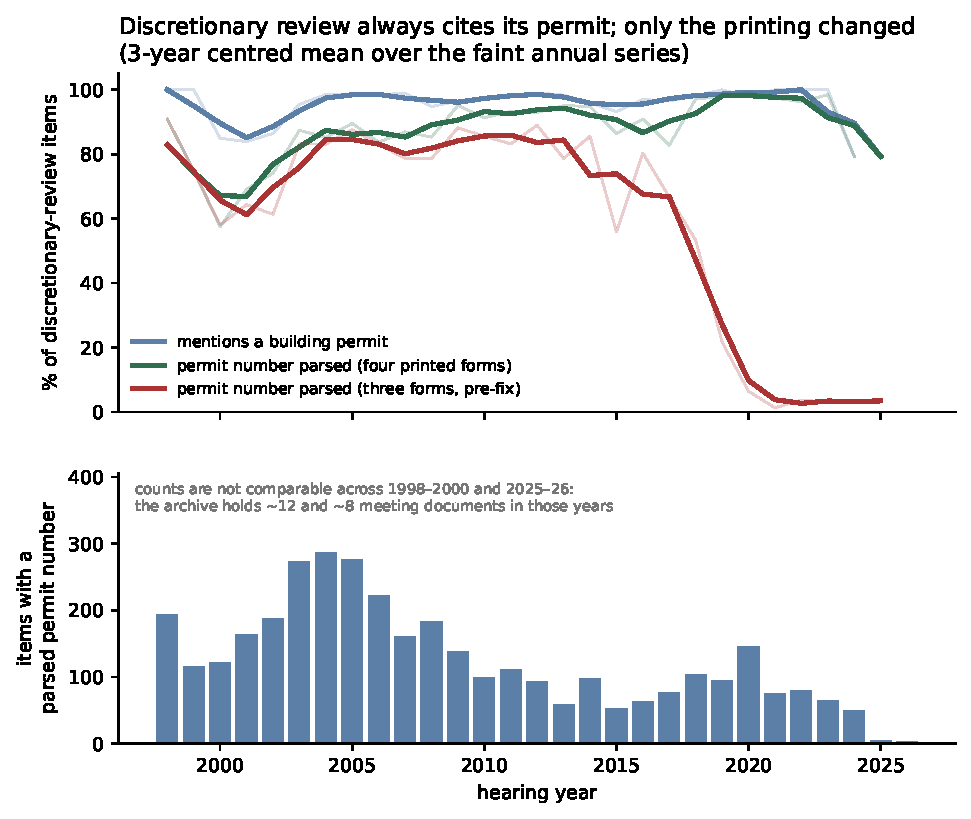
\includegraphics[width=\textwidth]{figures/fig_permit_coverage.pdf}
\caption{Discretionary-review items citing a permit, and the share from which a number can be
parsed, with and without the fourth printed form. Rates are suppressed for 2025 and 2026, in
which the archive holds 7 and 14 discretionary reviews respectively --- the scrape reached
the archive before the archive reached the present.}
\label{fig:coverage}
\end{figure}

Before this memo, the parsed-permit counts thinned to nothing after 2019: on discretionary
reviews, 9 items in 2020, 1 in 2021, 3 in 2022. Three explanations were possible --- the modern minutes dropping permit
numbers from the text, the collapse of discretionary review removing the items that carry
them, or a parsing failure on a newer printed format. Figure~\ref{fig:coverage} separates
them, and it is the third.

The blue line is the share of discretionary-review items that mention a building permit at
all. It sits between 95\% and 100\% from 2003 to 2024. The minutes never stopped printing the
permit. Nor did the items disappear: the Commission heard 140 discretionary reviews in 2020
and 81 in 2022, well within its historical range even after the post-2013 decline in the DR
share of the docket. What changed is the printing. From roughly 2017 the modern minutes
render the permit as \texttt{2019.0618.3775} --- year, MMDD, serial --- with two separators
where the older \texttt{2013.10.21.9832} has three. A regex written against the older form
matches none of them, and the red line falls off a cliff it did not have to.

Adding the two-separator form (\texttt{YYYY.MMDD.NNNN}) recovers \textbf{711 items and 483
distinct permits}, at a 98.0\% DBI match rate. Among discretionary reviews, parsed-permit
coverage in 2020 goes from 9 items to 139, in 2021 from 1 to 75, in 2022 from 3 to 78. The
permit route is usable for recent years, which is the years the paper most needs.

This is worth stating as a methodological point rather than a bug fix. The minutes are an
archive assembled by a department that changed its word processor several times in
twenty-eight years, and a deterministic rule that encodes one era's formatting silently
reports the other era as missing data. The check that caught it was cheap: measure the
\emph{mention} rate alongside the \emph{parse} rate, and any gap between the two is a parser
problem rather than a world problem. That pairing should be standard in this pipeline.

\section{Which parts of the docket the permit route reaches}

Table~\ref{tab:permitbytype} cross-tabulates against \texttt{request\_type}, and the answer is
sharp enough to be worth being explicit about: \textbf{the permit route is a discretionary-review
route}.

\begin{itemize}
\item \textbf{Discretionary review}: 4{,}117 items, 95.2\% cite a permit, 85.5\% yield a
number, 83.8\% match in DBI. This is expected --- a discretionary review \emph{is} a review of
a filed building permit, so the permit number is the subject of the hearing --- but the
magnitude is the useful part.
\item \textbf{Everything else}: at most 2\% on any other family, and below 0.5\% on
conditional use, the largest single request type at 5{,}074 items. A conditional use is an
authorisation to make a use of land; the building permit, if any, is filed afterwards and
under a different number. The minutes have nothing to cite.
\end{itemize}

So the permit-number join buys a near-complete construction-outcome panel for one quarter of
the docket, and nothing at all for the legislative, CEQA and historic families. Any analysis
built on the permit join is conditioned on being a discretionary review, and inherits
discretionary review's own selection --- small infill projects with a neighbour objecting.

\section{What the match buys}

\begin{figure}[htbp]\centering
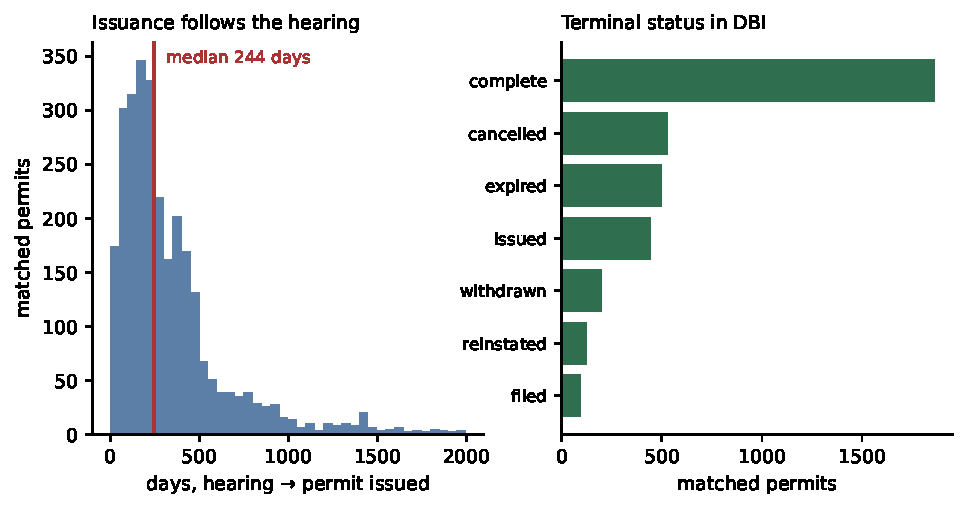
\includegraphics[width=\textwidth]{figures/fig_permit_outcomes.pdf}
\caption{For the 3{,}801 matched item--permit pairs: elapsed days from the hearing to permit
issuance (left, truncated at 2{,}000 days), and the permit's terminal status in DBI (right).}
\label{fig:outcomes}
\end{figure}

Table~\ref{tab:permitbuys} inventories what becomes observable. For a matched item:

\begin{itemize}
\item \textbf{The permit issued in 78.5\% of cases}, a median of \textbf{245 days} after the
hearing and 768 days at the 90th percentile. The hearing is not the end of the clock; it adds
most of a year to it, and the right tail of that addition is as wide as the delay inside the
hearing process itself.
\item \textbf{Construction started for 38.5\%}, dated by
\texttt{first\_construction\_document\_date}. That is the closest thing in the record to
``something was actually built''.
\item \textbf{32.9\% were withdrawn, expired, cancelled, revoked or disapproved} and 48.9\%
completed. The abandonment states are the observable trace of a project that lost its bet ---
the outcome the corpus memo identifies as the only route to the selection problem, since
projects never filed leave no record anywhere.
\item \textbf{Cost is recorded on 88.8\%} (median revised cost \$350{,}000) and
\textbf{proposed dwelling units on 84.8\%}.
\item \textbf{Supervisor district on 99.9\%}, which is the cheapest available route to a
political geography for the item table --- the minutes print a district only in the modern
era, and DBI prints one for essentially every permit.
\end{itemize}

The one comparison that does not work is units proposed at the hearing against units in DBI.
The extraction schema has no unit-count field, and a regex over the request text recovers one
for only 42 of the matched items, of which 57.1\% agree with DBI exactly. That is too thin to
be a validation of anything. It is not a defect of the join: discretionary reviews are
predominantly additions and alterations to existing houses, and the minutes describe the work
rather than counting units. If a unit count is wanted at the item level, DBI's
\texttt{proposed\_units} on the matched subset is a better source than the minutes text.

\section{The parcel route, scored honestly}

For the three quarters of the docket with no printed permit number, the fallback is the
parcel: 84.1\% of items carry an assessor block and at least one lot, and DBI keys every
permit the same way. The difficulty is that a parcel is not a project. The median matched
parcel carries about ten permits, most of them over-the-counter alterations --- 973{,}920 of
DBI's 1.3 million rows are \texttt{otc alterations permit} --- and picking the wrong one
attaches the wrong outcome to the hearing.

The permit-number subset is the ground truth for testing a rule, because on those items we
know which permit the hearing was about. Table~\ref{tab:parcelrule} scores seven rules on the
3{,}274 such items whose cited permit is present at the parcel DBI records for it. Coverage
(does the rule return anything?), precision (of what it returns) and recall (of what it should
have found) are reported separately, because a rule that returns nothing has undefined
precision and reporting it as zero flatters the wide rules.

The shape of the trade-off is clear. Taking every permit at the parcel has perfect recall and
0.14 precision --- six wrong permits for each right one. Restricting to new construction,
wood-frame new construction, alterations and demolitions --- dropping over-the-counter work
and signs --- raises precision to 0.44 at almost no cost in recall, and is the single most
valuable filter. Adding a date window trades recall for coverage: \textbf{filings from three
years before to one year after the hearing return a candidate set for 94.0\% of items, at
0.72 precision and 0.92 recall, with a median set size of one}. Tightening to one year before
and six months after raises precision only to 0.75 while dropping coverage to 56\% --- the
permit is often filed long before the hearing that reviews it, which is the whole reason a
discretionary review exists.

Taking only the nearest filing gives point identification at 0.74 precision and 0.67 recall.
That is the right rule if the analysis needs one permit per item and can tolerate a third of
them being wrong; the three-year window, whose candidate set has a median size of one, is the right rule if
the analysis can carry a set, for instance by taking the maximum project size or the earliest
issuance across candidates.

Table~\ref{tab:parcelreach} gives the reach. Of the 12{,}611 items with no printed permit
number, 10{,}076 have a block and lot, 9{,}455 have a parcel DBI knows, and \textbf{6{,}664
--- 41.1\% of the whole docket --- get at least one candidate permit} under the preferred
rule. Combined with the 3{,}515 items matched on a printed number, some construction-side
observation is available for \textbf{10{,}179 items, 62.8\% of the docket}, of which a little
over a third is exact and the rest is a small candidate set with a known error rate.

This is a positive result but it should not be oversold. The 0.72 precision is measured on
discretionary reviews, because that is where the ground truth is, and discretionary reviews
concern parcels with a specific pending permit. On a conditional-use item --- a restaurant
seeking a use authorisation on a busy commercial block --- the parcel's permit history is
denser and less related to the hearing, and the rule will do worse. Extending the validation
there requires ground truth that does not currently exist.

\section{Conditions of approval are not in DBI}

The corpus memo left open whether the conditions the Commission attaches at the hearing can be
recovered from the permit record. They cannot.

DBI's \texttt{description} field is populated on 98.6\% of rows and describes the
\emph{work}: ``install aluminum windows'', ``infill right side lightwell. remodel (e) kitchen
and add a new bathroom on 2/f of (e) building''. Searching all
1{,}295{,}048 rows for any mention of a condition of approval, a Planning Commission motion,
or work performed pursuant to one returns \textbf{87 rows --- 0.007\%}. There is no field for
planning conditions, and the free text does not carry them as a matter of practice. This is
not a coverage gap that better matching would close; DBI records the permit's own scope and
status because that is what a building department regulates.

The consequence is that the conditions question has to be answered somewhere else, which is
what the companion memo on conditions of approval takes up. The permit record answers
``what happened to the project'', not ``what was the project made to do''.

\section{What this establishes, and what it does not}

\textbf{Established.}
\begin{enumerate}
\item The permit-number join is a census, not a sample, and it holds at 97.6\% across all four
printed forms and all four decades.
\item The route is alive for 2017--2026; the earlier appearance of collapse was a parser
artefact, now fixed and regression-visible in Figure~\ref{fig:coverage}.
\item The join is a discretionary-review instrument. It reaches 83.8\% of DR items and under
2\% of everything else.
\item For matched items, issuance, construction start, abandonment, cost, units and
supervisor district are all observable, with issuance a median 245 days after the hearing.
\item A parcel-plus-window-plus-type rule extends partial coverage to a further 41\% of the
docket at 0.72 precision and 0.92 recall, validated against the permit-number subset.
\item Conditions of approval are absent from DBI.
\end{enumerate}

\textbf{Not established.}
\begin{enumerate}
\item Whether the parcel rule's precision survives outside discretionary review. It is
measured where the ground truth is, and that is not a random part of the docket.
\item Whether an unmatched permit number means the permit does not exist or the minutes
mis-transcribed it. 56 numbers, small enough to adjudicate by hand, and worth doing before
any analysis treats non-match as an outcome.
\item Whether \texttt{proposed\_units} in DBI is the right unit count for a project that was
modified at the hearing. DBI records the permit as filed and as revised; which revision
post-dates the Commission's action is knowable from \texttt{status\_date} but has not been
checked.
\item Anything causal. The 245-day median lag from hearing to issuance is a description of a
joined record, not an estimate of what the hearing did to the clock.
\end{enumerate}

\section{Reproducing this}

\texttt{code/commission\_minutes\_processing/analyze\_permits.py} does all of it: it caches
DBI (\texttt{-{}-refresh} to re-download), parses, matches, scores the parcel rules, writes
both figures and \texttt{tables/permit\_tables.tex}, and emits two artefacts next to the
extraction on Dropbox --- \texttt{permit\_matches.csv}, one row per (item, cited permit) with
the DBI fields attached, and \texttt{permit\_summary.json}, which
\texttt{analyze\_corpus.py} reads so the corpus memo's linkage table cannot drift from this
one. No number in this memo is hand-placed.

\end{document}
